\documentclass[xcolor=dvipsnames]{beamer}

\usepackage{stmaryrd}
\usepackage{amssymb,amsthm,amsmath,amsxtra}
\usepackage{tikz}
\usetikzlibrary{arrows,calc,automata,shadows,backgrounds,positioning,intersections,fadings,decorations.pathreplacing,shapes,snakes, matrix}
\usepackage{tikz-cd}
\usepackage{diagbox}
\usepackage{eso-pic}
\usepackage[all]{xy}
\usepackage{colonequals}
\hypersetup{colorlinks=true,urlcolor=blue,citecolor=blue,linkcolor=blue}

\usepackage{beamerthemesplit}
\usecolortheme[named=Green]{structure} 
% \usetheme{Singapore}
% \setbeamersize{text margin top=-1in}
\setbeamertemplate{navigation symbols}{}%remove navigation symbols

\addtolength{\parskip}{0.5\baselineskip}
\setlength{\arraycolsep}{2pt}

\DeclareMathOperator{\area}{area}
\DeclareMathOperator{\opchar}{char}
\DeclareMathOperator{\opdiv}{div}
\DeclareMathOperator{\grad}{grad}
\DeclareMathOperator{\Cl}{Cl}
\DeclareMathOperator{\disc}{disc}
\DeclareMathOperator{\Gal}{Gal}
\DeclareMathOperator{\M}{M}
\DeclareMathOperator{\tr}{tr}
\DeclareMathOperator{\nrd}{nrd}
\DeclareMathOperator{\opP}{P}
\DeclareMathOperator{\OO}{O}
\DeclareMathOperator{\PGL}{PGL}
\DeclareMathOperator{\GL}{GL}
\DeclareMathOperator{\PSL}{PSL}
\DeclareMathOperator{\PSU}{PSU}
\DeclareMathOperator{\SL}{SL}
\DeclareMathOperator{\SO}{SO}
\DeclareMathOperator{\vol}{vol}
\DeclareMathOperator{\hht}{ht}

\newcommand{\quat}[2]{\displaystyle{\biggl(\frac{#1}{#2}\biggr)}}

\theoremstyle{plain}
\newtheorem*{thm}{Theorem}
\newtheorem*{prop}{Proposition}
\newtheorem*{cor}{Corollary}
\newtheorem*{conj}{Conjecture}
\newtheorem*{ques}{Question}

\newcommand{\psmod}[1]{~(\textup{\text{mod}}~{#1})}

\newcommand{\C}{\mathbb C}
\newcommand{\F}{\mathbb F}
\newcommand{\HH}{\mathbb H}
\newcommand{\PP}{\mathbb P}
\newcommand{\R}{\mathbb R}
\newcommand{\Q}{\mathbb Q}
\newcommand{\Z}{\mathbb Z}
\newcommand{\Qbar}{\overline{\mathbb Q}}
\newcommand{\calD}{\mathcal{D}}
\newcommand{\calG}{\mathcal{G}}
\newcommand{\calH}{\mathcal H}
\newcommand{\calO}{\mathcal O}

\newcommand{\scrE}{\mathcal E}

\newcommand{\frakp}{\mathfrak p}

\usepackage{booktabs}

\newcommand{\defi}[1]{\textbf{#1}} 				% for defined terms

\setlength{\hfuzz}{4pt}

\newcommand{\legen}[2]{\left(\frac{#1}{#2}\right)}

\title{The $L$-functions and Modular Forms DataBase (LMFDB)}
\author{John Voight \\ Dartmouth College}
\date{Simons Collaboration on Arithmetic Geometry, \\
Number Theory and Computation \\ Annual Meeting \\ Simons Foundation, NYC \\ 10 January 2019}

\begin{document}

\begin{frame}[plain]
\titlepage
\end{frame}

\begin{frame}[plain]
\frametitle{Outline of this talk} \pause

\begin{enumerate}
\item (Re)Introduce the LMFDB;
\item New classical modular forms functionality \\ (private screening/world premiere!);
\item Future plans.
\end{enumerate}
 
\end{frame}

\begin{frame}[plain]
\frametitle{The LMFDB, in a nutshell} \pause

The LMFDB is a catalogue of mathematical objects arising in connection with the Langlands program, including  \pause 
\begin{center}
modular forms, $L$-functions, number fields, zeta zeros, elliptic curves, Maass forms, Artin representations, genus 2 curves, ... \pause
\end{center}

The LMFDB was first conceived at an AIM workshop in 2007.  \pause  The acknowledgements list 100 contributors.  \pause It has received substantial funding by the NSF, EPSRC, and the Simons Foundation, in addition to other smaller grants.  \pause  (Thank you!)   \pause

It is now managed like a journal, with managing editors (John Cremona, John Jones, Drew Sutherland, and me) and a team of associate editors.
\end{frame}

\begin{frame}[plain]
\frametitle{Motivation and desiderata} \pause

\begin{itemize}
\item Number theory has historically been in part an experimental science: even Gauss used tables of primes.  \pause  Big databases are now ubiquitous in science.  \pause
\item By exhaustive computation, we can catch some issues (``sweep in all corners'') and bugs in code (``compute all examples''). \pause
\item Databases should be easily accessible online.  \pause  (Not easy if data is scattered on homepages: learn format, install program, ...  Worse still if a paper says ``E-mail me if you want the data''.) \pause 
\item Data sets should be connected to one another.  \pause (Sometimes the point is to make connections across data sets.) \pause
\item Data should be reliable and have a glossary/appropriate annotations. \pause
\item Data should be searchable, so you can find particular examples of interest. \pause (Before you prove something, it's helpful to know if there are counterexamples!) \pause
\item Data should have statistics, to notice patterns in aggregate.
\end{itemize}
\end{frame}

\begin{frame}[plain]
\frametitle{Technical specs} \pause

\begin{itemize}
\item Size: The LMFDB includes a database of zeros of $\zeta(s)$ (1 TB), class groups of imaginary quadratic fields (2 TB), with the rest of the data totalling 600+ GB.  \href{http://cmfs.lmfdb.xyz/api/stats}{More detailed stats} are available. \pause
\item The LMFDB is currently hosted in the Google cloud rather than on a university-hosted server.  \pause
\item The underlying database will soon be PostgreSQL, an object-relational database management system.  \pause  (We moved from MongoDB, which is a document database; talk to Edgar Costa and David Roe for more details!)  
\end{itemize}
\end{frame}

\begin{frame}[plain]
\frametitle{Big picture} \pause

\begin{center}
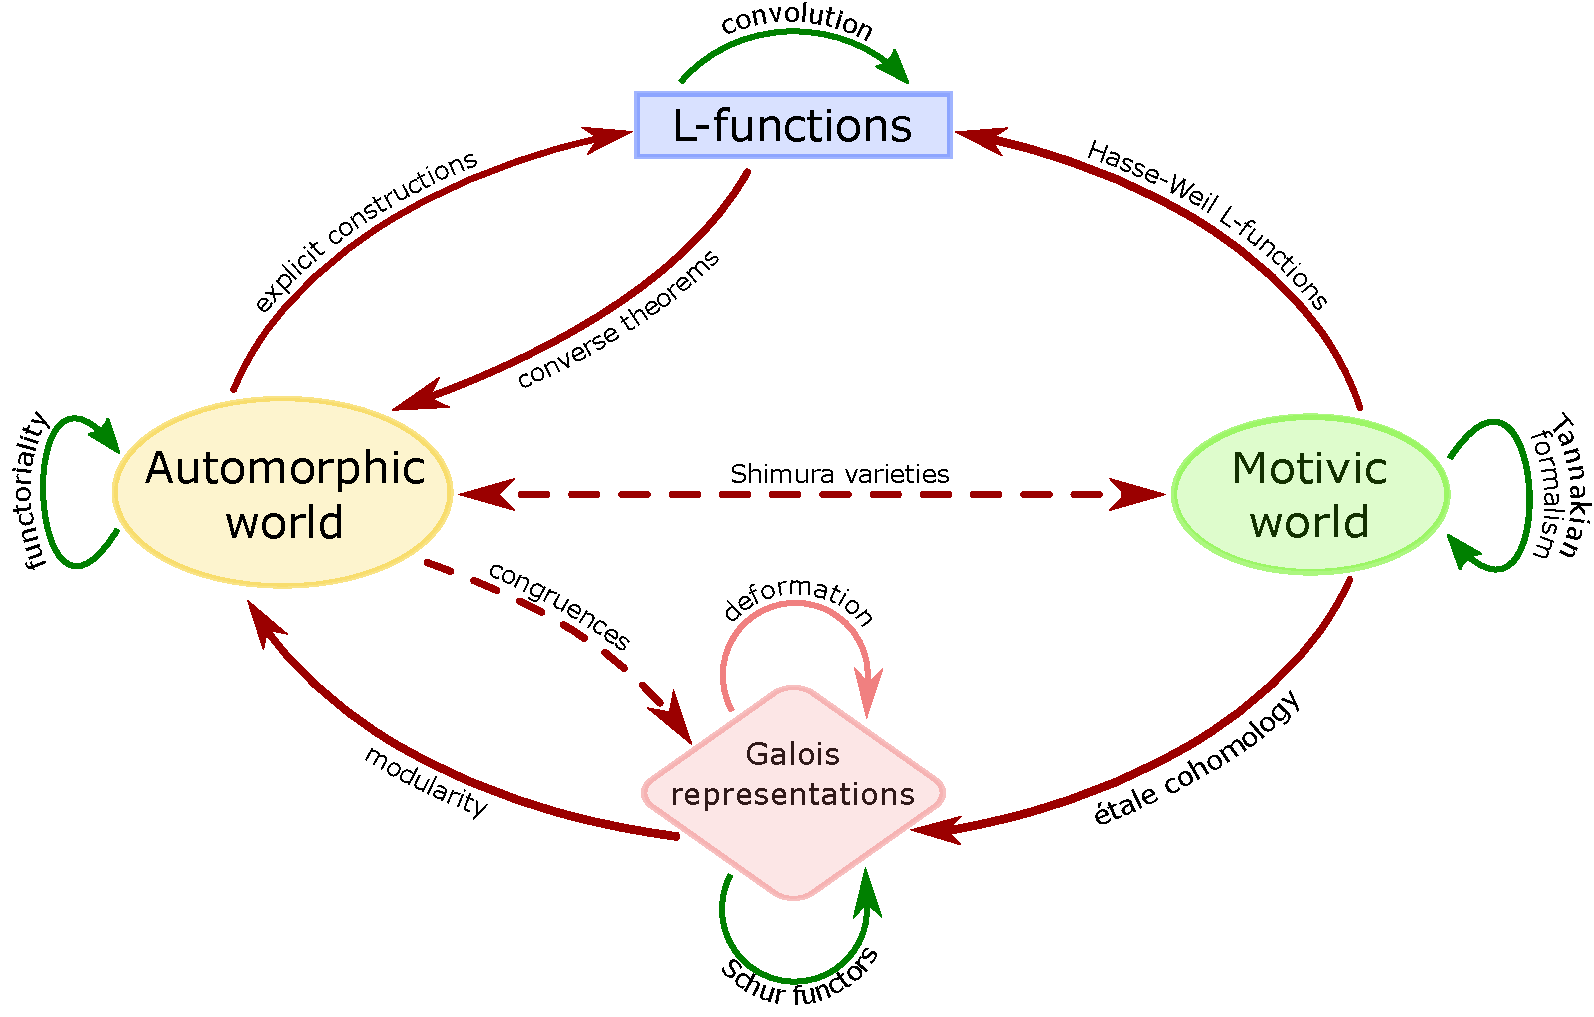
\includegraphics[width=4in]{lmfdbmap.pdf} \\
\href{http://www.lmfdb.org/universe}{LMFDB Universe}
\end{center}

\end{frame}

\begin{frame}[plain]
\frametitle{Classical modular forms} \pause

At a week-long workshop in August at MIT funded by the Simons Foundation, a significant upgrade was made to the MFs in the LMFDB.  \pause  Edgar Costa and David Roe (Simons postdocs at MIT, led by Drew Sutherland) have continued the charge through this year.  \pause  Thanks to Alex Best, Jonathan Bober, Andy Booker, John Cremona, and David Lowry-Duda.  \pause

\begin{center}
\includegraphics[width=3in]{2018-08-27.pdf}
\end{center}

\end{frame}

\begin{frame}[plain]
\frametitle{History: Wada 1971} \pause

\begin{center}
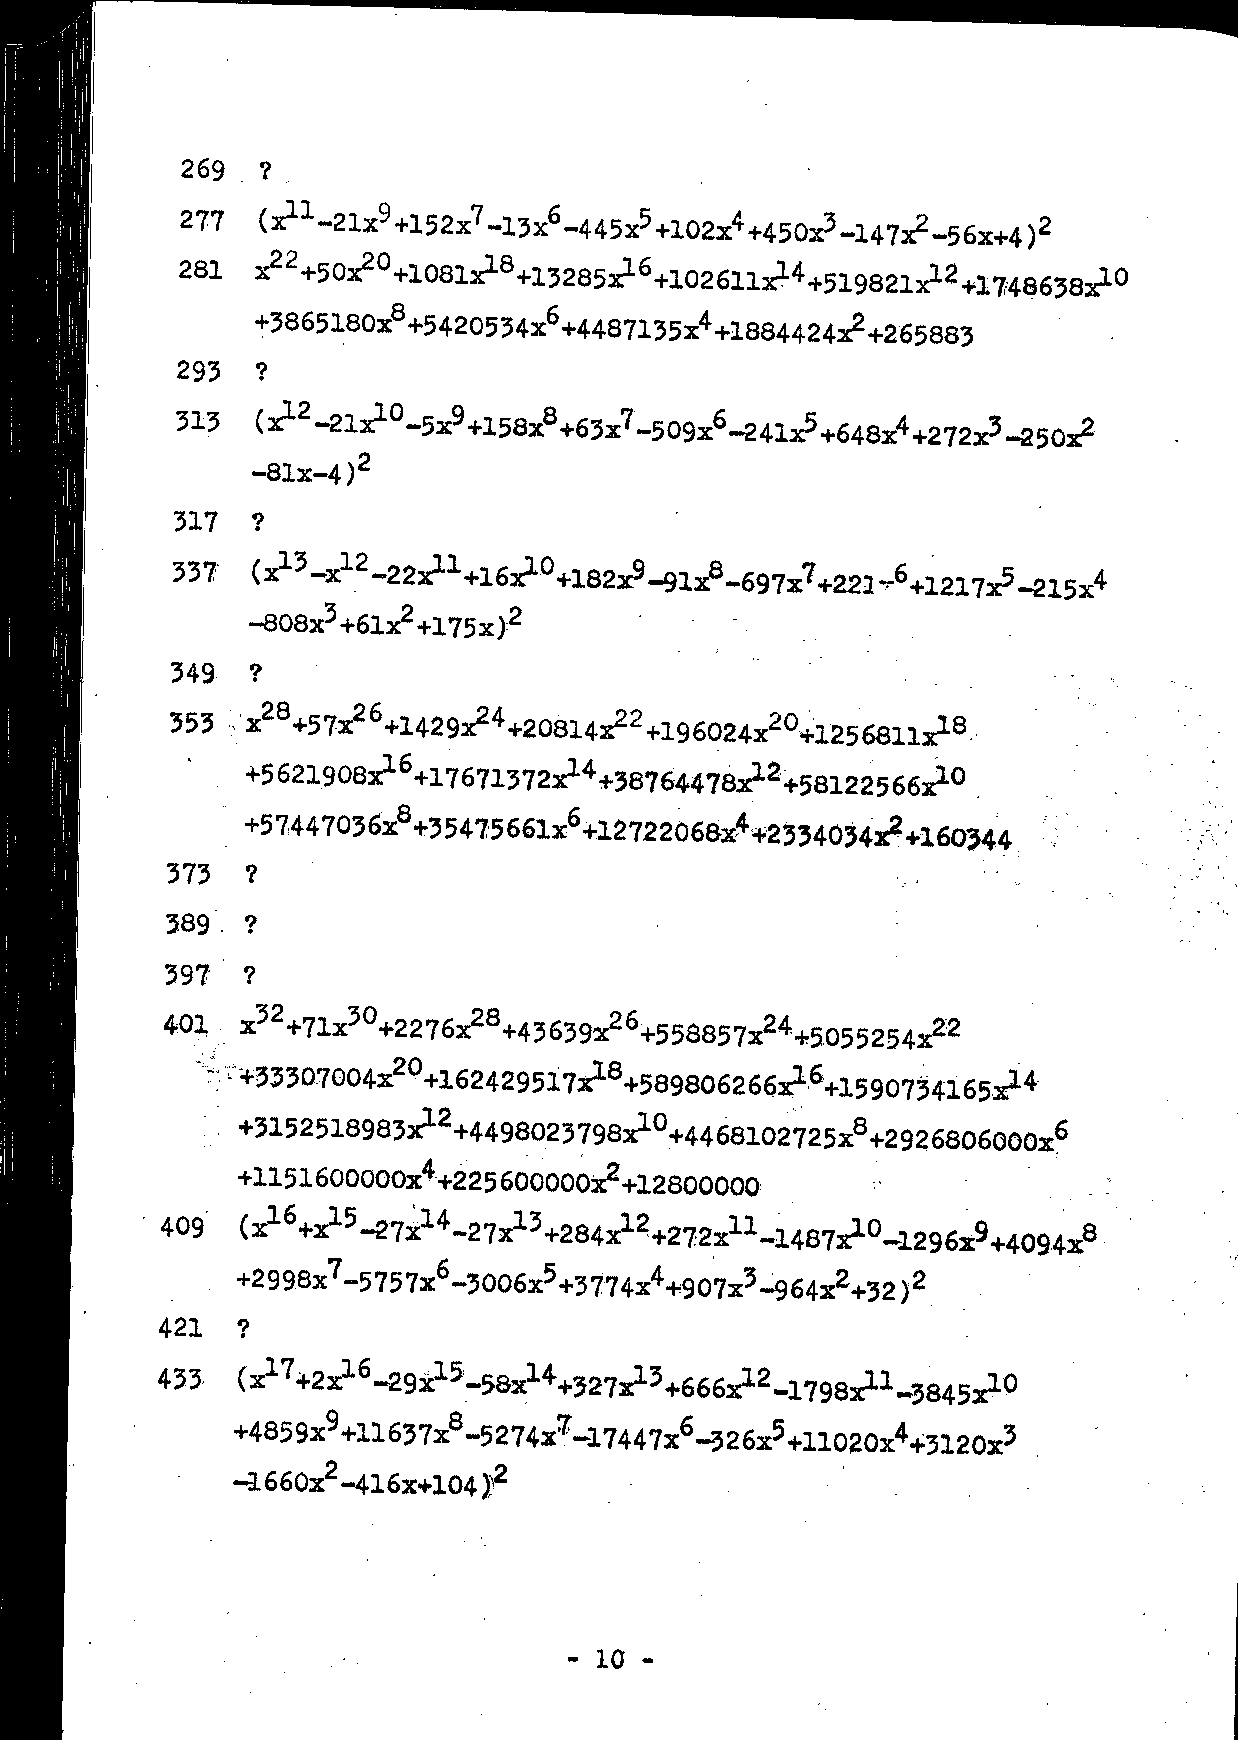
\includegraphics[width=3in]{Wada.pdf}
\end{center}

\end{frame}

\begin{frame}[plain]
\frametitle{History: Antwerp IV 1975} \pause

\vspace{-0.15in}
\begin{center}
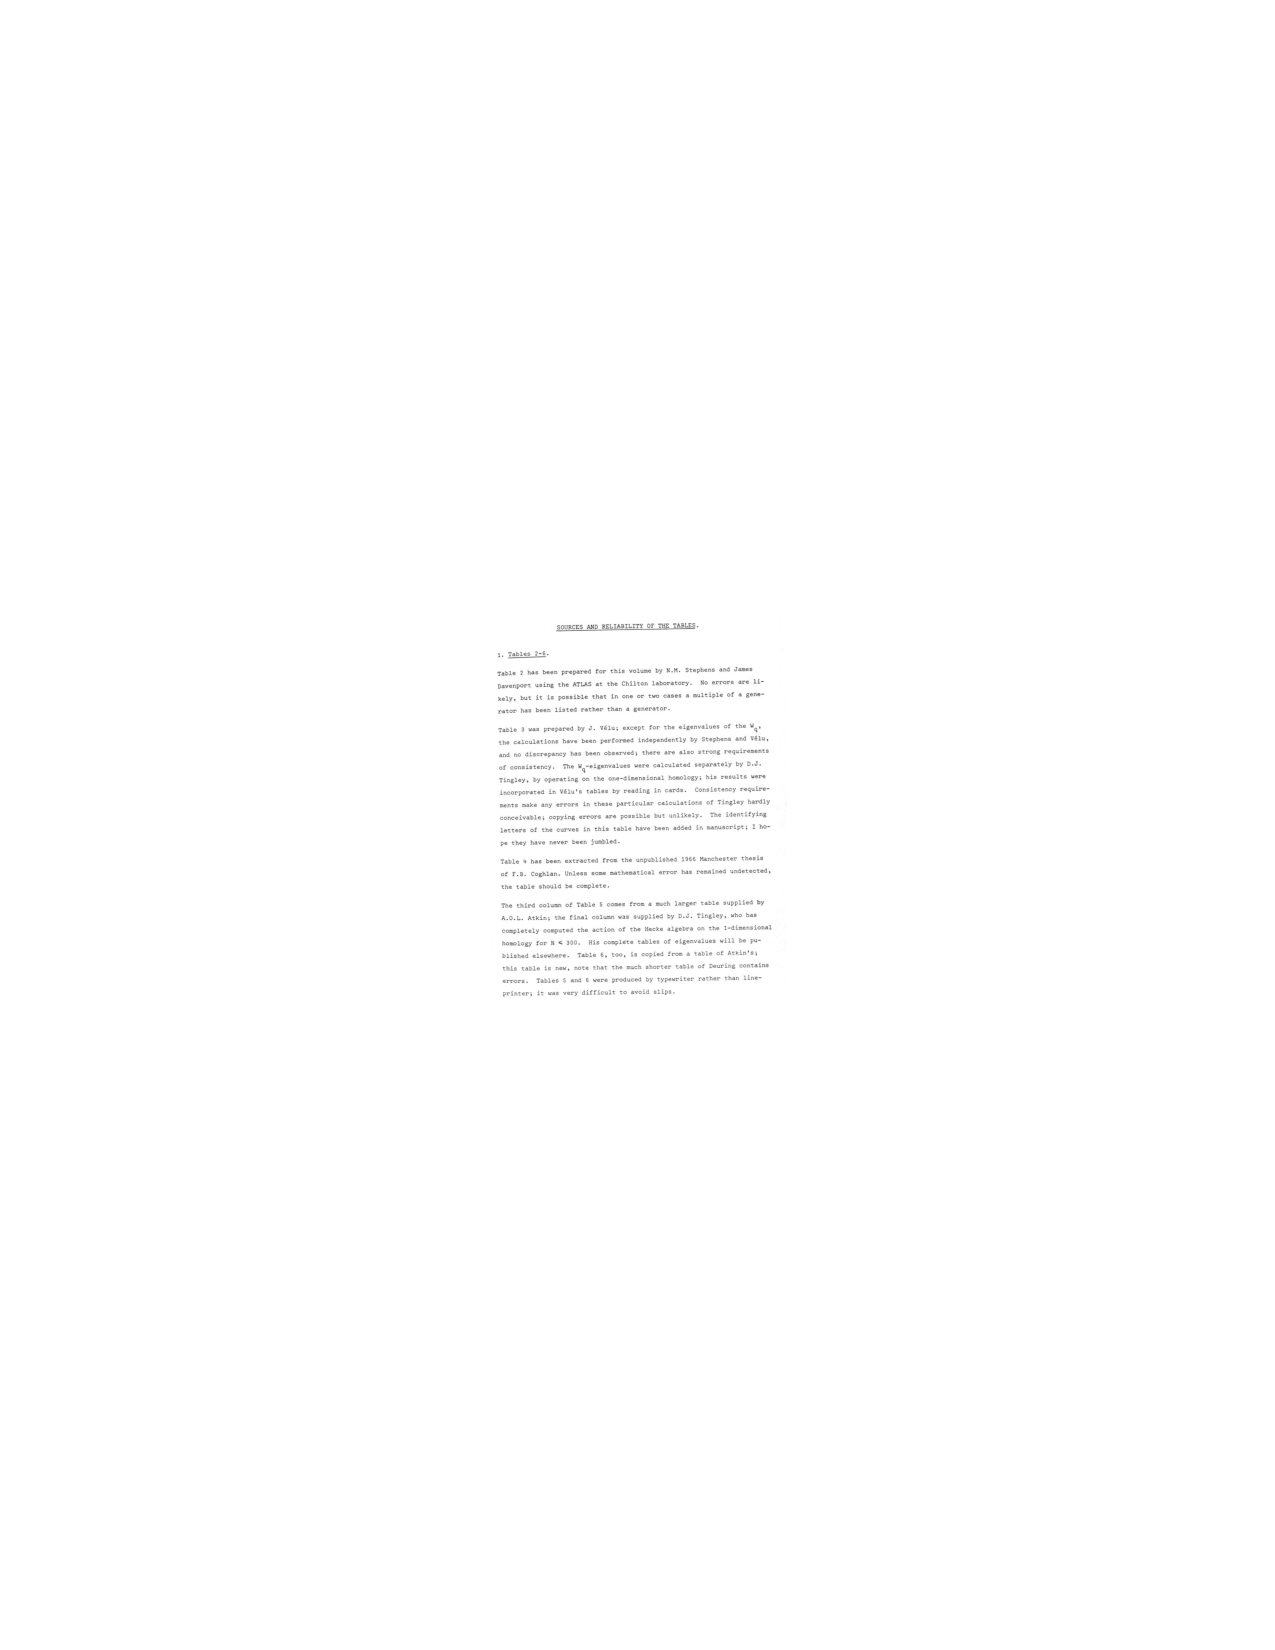
\includegraphics[width=2.6in]{antwerpiv.pdf} 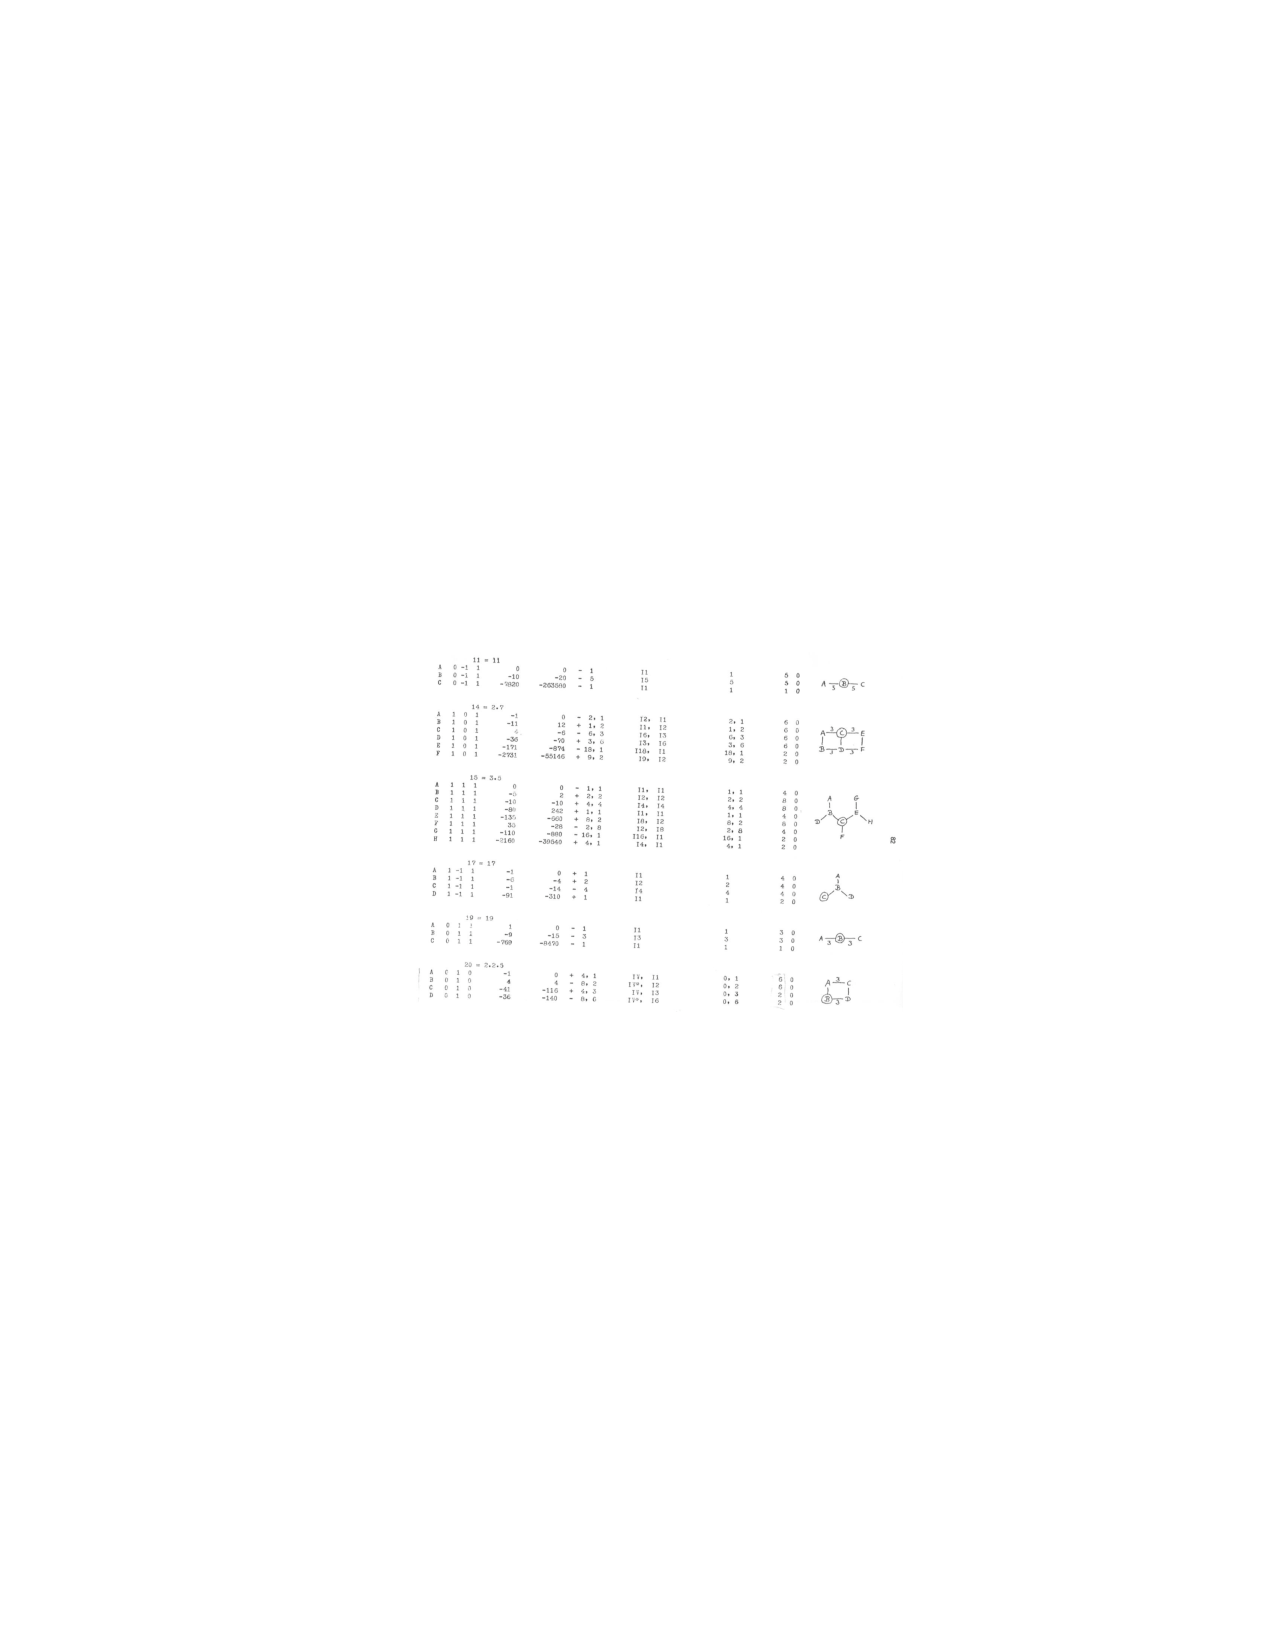
\includegraphics[width=4in]{antwerpiv1.pdf}
\end{center}
\end{frame}

\begin{frame}[plain]
\frametitle{Stein 2000s} \pause

\begin{center}
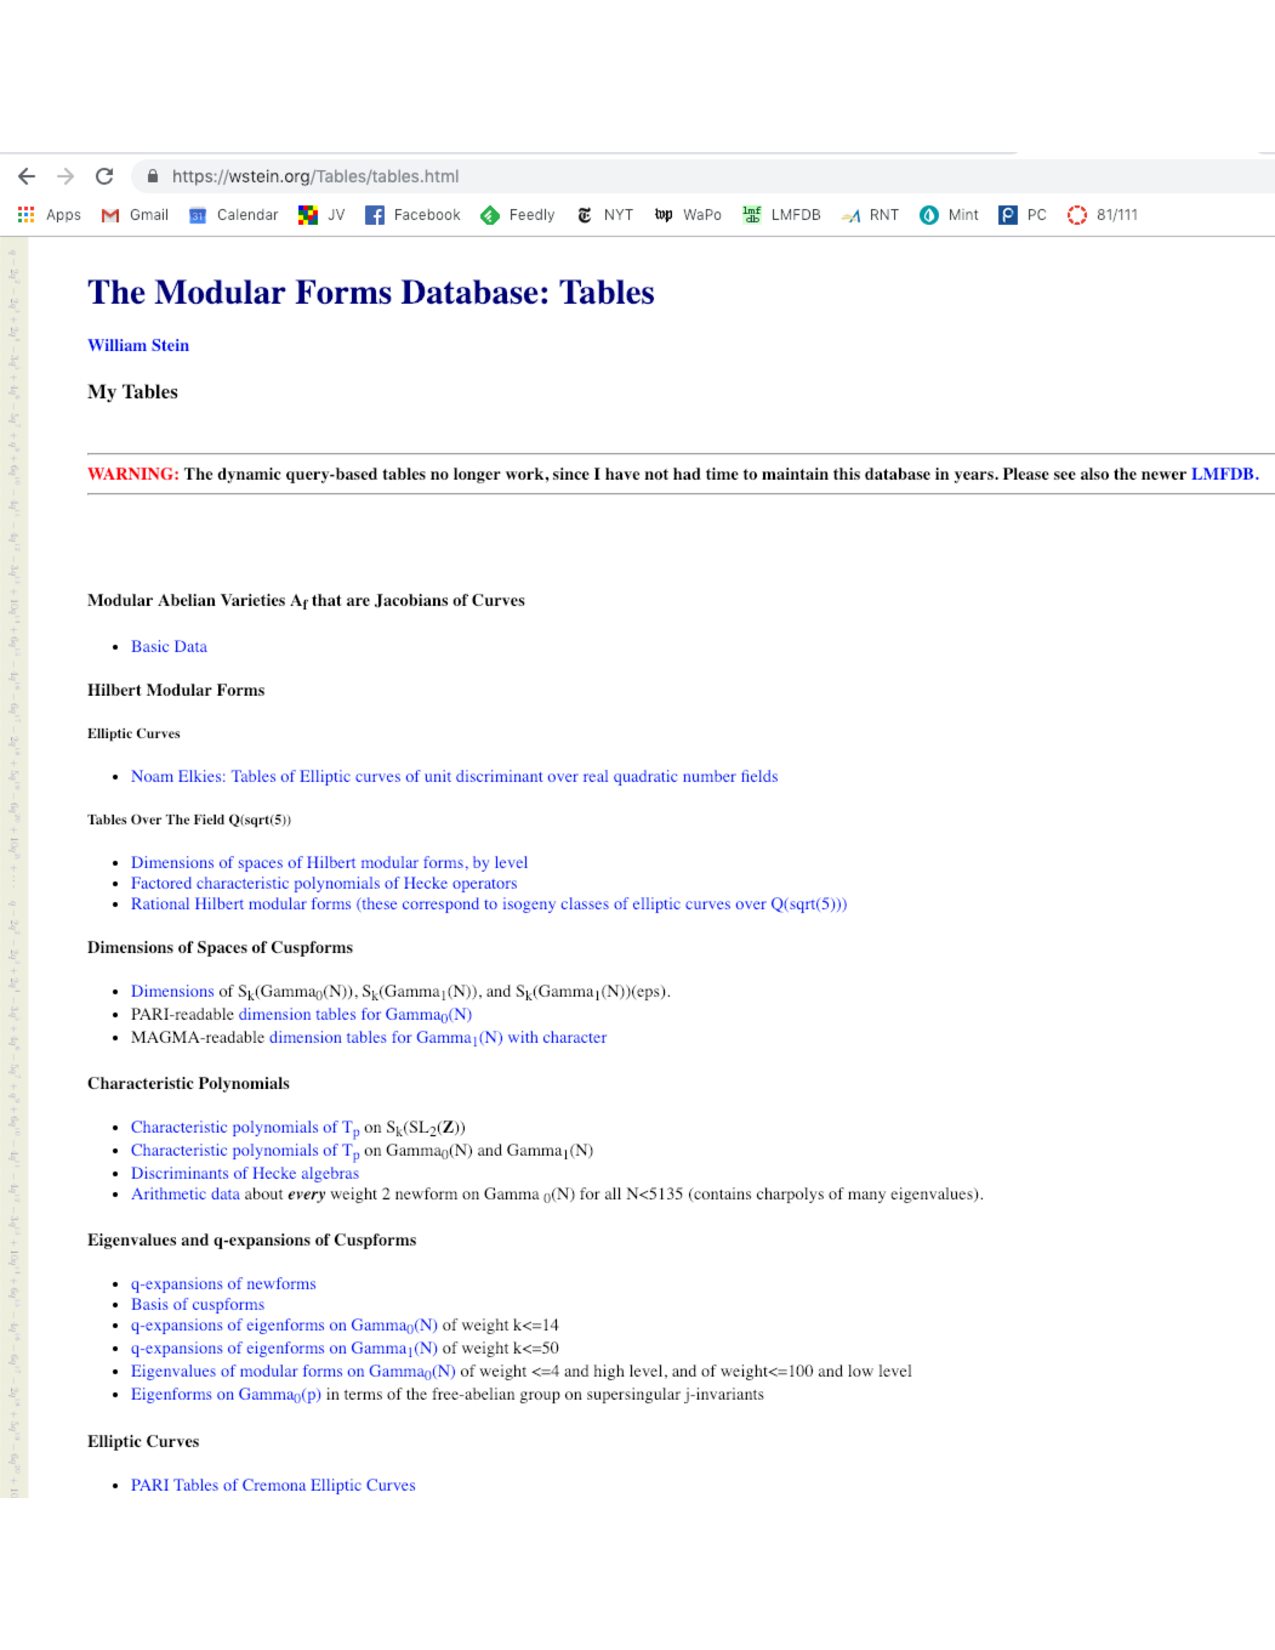
\includegraphics[width=2.6in]{stein.pdf} \\
\href{https://wstein.org/Tables/tables.html}{Stein tables}
\end{center}

\end{frame}

\begin{frame}[plain]
\frametitle{LMFDB: Scope of data} \pause

To be systematic, our data includes two big ``boxes'':  \pause
\begin{itemize}
\item All spaces $S_k(\Gamma_1(N))$ with $N,k \in \Z_{\geq 1}$ and $Nk^2 \leq 4000$, \pause and
\item All spaces $S_k(\Gamma_0(N))$ with $N,k \in \Z_{\geq 2}$ and $Nk^2 \leq 40000$ (trivial character). \pause
\end{itemize}

With additional boxes to cover the spread, we easily majorize Stein's database (and current LMFDB offerings).  \pause

Data computed using Magma, Pari, and code of Bober--Booker. \pause

\begin{itemize}
\item Data for 316\,236 newspaces $S_k(\Gamma_0(N),\chi)$ (50\,098 nonzero) \pause
\item $236\,555$ (Galois orbits of) newforms (48\,324 with rational coefficients, 19\,306 weight 1) \pause
\item $13\,710\,564$ complex embedded newforms \pause
\item Total size (including $L$-functions) about 300 GB \pause
\end{itemize}

\href{http://cmfs.lmfdb.xyz/ModularForm/GL2/Q/holomorphic/}{Search page} and 
\href{http://cmfs.lmfdb.xyz/ModularForm/GL2/Q/holomorphic/11/2/a/a/}{11.2.a.a} (to show homepages)
\end{frame}

\begin{frame}[plain]
\frametitle{A sampling of new features (items 1--5)} \pause

\begin{enumerate}
\item We bound our boxes by $Nk^2$, which is a good approximation to the analytic conductor $N\lvert\lvert k \rvert\rvert^2$ which governs the total complexity of the $L$-function (for more, talk to David Roberts).  \pause  In particular, our data is complete in these boxes.  \href{http://cmfs.lmfdb.xyz/ModularForm/GL2/Q/holomorphic/}{Search page} \pause 
\item Coefficients $a_n$ are represented compactly: either sparse cyclotomic (\href{http://cmfs.lmfdb.xyz/ModularForm/GL2/Q/holomorphic/1620/1/bp/a/}{1620.1.bp.a}) or \pause 
in terms of an LLL-reduced basis for the Hecke ring (\href{http://cmfs.lmfdb.xyz/ModularForm/GL2/Q/holomorphic/6877/2/a/s/}{6877.2.a.s}). \pause
\item We have complex eigenvalues when exact eigenvalues would be computationally infeasible (\href{http://cmfs.lmfdb.xyz/ModularForm/GL2/Q/holomorphic/983/2/c/a/}{983.2.c.a}), allowing for the computation of all $L$-functions, and can customize the display the embeddings (\href{http://cmfs.lmfdb.xyz/ModularForm/GL2/Q/holomorphic/2412/1/b/b/}{2412.1.b.b}). \pause
\item Self-twists (all rigorously proved), inner twists (indicated when proved or not), Atkin-Lehner eigenvalues, Hecke cutters available (\href{http://cmfs.lmfdb.xyz/ModularForm/GL2/Q/holomorphic/441/4/a/p/}{441.4.a.p}). \pause
\item Can download the form to get more coefficients, reduce, ...
\end{enumerate}
\end{frame}

\begin{frame}[plain]
\frametitle{Item 6: Trace tables (matching classical modular forms)} \pause

{\footnotesize\tt
Dear John, please forgive a cold call.

With colleagues, I have been calculating local zeta functions for Calabi-Yau varieties in a family depending on t. In general this gives rise to a factor

$1 + a T + b p T^2 + a p^3 T^3 + p^6 T^4$.

For $t=33\pm 8 \sqrt{17}$, the quartic factors in the form

$(1 - \alpha p T + p^3 T^2) (1 - \beta T + p^3 T^2)$

whenever $17$ is a square mod $p$.

We have lists  of data of the form $p, t, \{\alpha, \beta\}$ for when this happens, and we believe that the coefficients $\{\alpha, \beta\}$ are coefficients of a (Hilbert) modular form. 

So finally I come to my question, which is: is there a practical way of extracting lists of coefficients of such modular forms from LMFDB with which to compare our lists? 

We have a number of cases similar to the example above so we hope for a simple procedure that we can repeat as necessary.

\ \\ }
\end{frame}

\begin{frame}[plain]
\frametitle{Narrowing the search} \pause

\begin{itemize}
\item There is bad reduction at $17$, and possibly at $2$.  \pause

\item The quartic factor is independent of the choice of $\sqrt{17}$ modulo $p$, so we guess that there is descent from $F=\Q(\sqrt{17})$ to $\Q$.  \pause

\item We guess that the Hodge structure splits as
\[ (1,1,1,1) = (0,1,1,0) + (1,0,0,1) \pause \]
and accordingly the (likely) $\ell$-adic Galois representation 
\[ \rho \colon \Gal_F \to \GL_4(\Q_\ell) \]
is the base change from $\Q$ to $F$ of 
\[ \rho_f(-1) \oplus \rho_g \]
where $f,g$ are classical modular forms of weights $2,4$. \pause
\item We have a fair amount of eigenvalue data:
\[ \begin{array}{c|ccccc} 
p & 13 & 19 & 43 & 67 & \cdots \\
\hline
a_p(f) & 2 & -4 & -4 & -4 & \cdots \\
a_p(g) & -42 & 60 & 508 & -676 & \cdots
\end{array} \]
Let's \href{http://cmfs.lmfdb.xyz/ModularForm/GL2/Q/holomorphic/}{search for the form}!
\end{itemize}

\ \\

\end{frame}

\begin{frame}[plain]
\frametitle{Item 7: Weight 1 forms} \pause

We treat weight 1 forms.  \pause 

\begin{enumerate}
\item[a.] The data set majorizes the Buzzard--Lauder database. \pause
\item[b.] The projective image types have been proved for all weight 1 forms, requiring a couple of new tricks.  \href{http://cmfs.lmfdb.xyz/ModularForm/GL2/Q/holomorphic/124/1/i/a/}{124.1.i.a} (smallest $A_4$), \href{http://cmfs.lmfdb.xyz/ModularForm/GL2/Q/holomorphic/148/1/f/a/}{148.1.f.a} (smallest $S_4$), \href{http://cmfs.lmfdb.xyz/ModularForm/GL2/Q/holomorphic/1763/1/p/b/}{1763.1.p.b} (new $A_5$); \href{http://cmfs.lmfdb.xyz/ModularForm/GL2/Q/holomorphic/3600/1/e/a/}{3600.1.e.a} ($D_2$, having RM and CM), \href{http://cmfs.lmfdb.xyz/ModularForm/GL2/Q/holomorphic/3997/1/cz/a/}{3997.1.cz.a} ($D_{285}$). \pause
\item[c.] Artin representations are matched whenever these were already present in the LMFDB. \href{http://cmfs.lmfdb.xyz/ModularForm/GL2/Q/holomorphic/385/1/q/b/}{385.1.q.b} \pause 
\item[d.] Dimension data for subspaces by projective image type.  \href{http://cmfs.lmfdb.xyz/ModularForm/GL2/Q/holomorphic/1161/1/i/}{1161.1.i}.  
\end{enumerate}

\end{frame}

\begin{frame}[plain]
\frametitle{A sampling of new features (items 8--10)} \pause

\begin{enumerate}
\item[8.] Can view dimension tables, with constraints.  For example, \href{http://cmfs.lmfdb.xyz/ModularForm/GL2/Q/holomorphic/?count=None&hidden_search_type=Dimensions&level=1-48&weight=1-12&dim=1&search_type=Dimensions}{rational forms}. \pause
\item[9.] Dynamic statistics: you can tabulate statistics for a specified subset of the data.  For example, what are the \href{http://cmfs.lmfdb.xyz/ModularForm/GL2/Q/holomorphic/dynamic_stats}{statistics} for weight and level for those forms having self-twist? \pause
\item[10.] Provable analytic ranks (including \href{http://cmfs.lmfdb.xyz/ModularForm/GL2/Q/holomorphic/?is_self_dual=no&count=50&analytic_rank=1&search_type=List}{non-self dual forms of analytic rank $1$}).  \pause  We found a rational form (\href{http://cmfs.lmfdb.xyz/ModularForm/GL2/Q/holomorphic/2/42/a/a/}{2.42.a.a}) of weight $42$ and a form (\href{http://cmfs.lmfdb.xyz/ModularForm/GL2/Q/holomorphic/8/14/b/a/}{8.14.b.a}) of weight $14$ each having analytic rank $1$.
\end{enumerate}

\end{frame}

\begin{frame}[plain]
\frametitle{Future plans} \pause

\begin{enumerate}
\item Annotations for interesting examples (IAS, March 2019). \pause
\item Think of the LMFDB as like an ``OEIS (Online Encyclopedia of Integer Sequences) for $L$-functions.''  \pause \\
$L$-functions can have many origins: \href{http://cmfs.lmfdb.xyz/L/EllipticCurve/2.2.56.1/32.1/c/}{2.2.56.1-32.1-c} has at least 12 origins! \pause
\item New data sets: mod $p$ Galois representations, Siegel paramodular forms, half-integer weight modular forms, hypergeometric motives, Belyi maps, small groups, ... \pause
\end{enumerate}

We hope the LMFDB will be a useful tool on your workbench!
\end{frame}

\end{document}